\section{Results}\label{sec:results}

\paragraph{Decision rules, fixed before the results.} A measure is usable if it scores most videos, a topic's own
video scores higher than another topic's video, and two measurements of the same videos agree. The learner repair
helps if it beats the generic repair of the same size; finding the weak section matters if it also beats rewriting
every section. A pipeline feature helps if it raises these differences without hurting the layout. All numbers are
means over topics on a 0--100 scale; paired bootstrap intervals and Wilcoxon tests are kept with the result files.
We call a difference \emph{beyond noise} only if it passes two tests. First, it must survive randomly swapping the two
versions' answers question by question. Second, its sign must hold across topics. The student is not fully
repeatable. We re-asked \NMRepeatN{} questions on identical frames, and its confidence in the right answer moved on
\NMRepeatMoved{} of them, a few times by up to half the scale. On one concept, repeat noise alone moves M9 by up to
\NMFloorOne{} points (95\%); on the mean of all concepts, by up to \NMFloorAll{}.

\paragraph{The ladder on MMMC} (Table~\ref{tab:ladder_mmmc}). Our analysis yields four insights.
(i) \textbf{The student already knows MMMC.} Forced to choose, it answers every question right with no video on
\LadMMMCBlindAllRight{} of \LadMMMCTopics{} pilot topics. There is nothing left to learn, so every gain measure
(M3--M9) scores \LadMMMCDefinedNVG{} videos.
(ii) \textbf{TeachQuiz sees the topic, not the repair.} With answers matched in order (M1), a topic's own video beats
another topic's video by \LadMMMCSepOne{} points, but the learner repair beats the base video by only
\LadMMMCLBOne{}, and \LadMMMCTiesOne{} of \LadMMMCTopics{} topics are ties. With forced choice (M2), all
\LadMMMCTiesTwo{} topics are ties.
(iii) \textbf{The raw scores sit at the prior ceiling.} Without normalisation, confidence in the right answer is
\LadMMMCSBlind{} with no video and \LadMMMCSVisual{} with the dense video. Another topic's video lowers it further,
which is all that the own-versus-other difference of R9 (\LadMMMCSepRawNine{}) measures.
(iv) \textbf{A smaller student does not change the picture.} With \texttt{qwen2.5vl:3b}, confidence with no video is
\LadSmallSBlind{}, so the gain on 3 frames per section (M9) scores \LadSmallDefinedNine{} videos
(Table~\ref{tab:ladder_small}). Its own video beats another topic's by \LadSmallSepNine{} points, but the learner
repair scores \LadSmallLBNine{} against the base video: each topic's gain rests on one or two questions. With so
little room left, a learner-versus-base difference would have to reach about \NMSmallMDE{} points before this design
could detect it.
On MMMC, with this student, the repair can neither succeed nor fail; the pilot's null result is not evidence
against it.

\begin{table*}[!tbp]\centering\footnotesize
\caption{A smaller student (qwen2.5vl:3b) on the MMMC pilot videos, 3 frames per section only; measures it could not score are left out. 12 topics, 48 videos. Each row adds one change to the row above; points on a 0--100 scale. The first three columns use each topic's base video only, since its repairs are near-copies of it. Scored: base videos that get a score (-- : the student already knew everything). Own $-$ other: a topic's video minus another topic's video on the same quiz. Agreement: rank correlation of two measurements of the same base videos. Learner $-$ \ldots: mean change over topics, the versions paired by topic. Ties: topics where learner and base score the same.}\label{tab:ladder_small}
\setlength{\tabcolsep}{4pt}\begin{tabular}{@{}llrrrrrrr@{}}\toprule & & \multicolumn{3}{c}{Does it measure teaching?} & \multicolumn{4}{c}{Does the learner repair help?}\\
\cmidrule(lr){3-5}\cmidrule(lr){6-9}
& Measure & Scored & \hd{Own $-$\\other ($\uparrow$)} & \hd{Agree-\\ment ($\uparrow$)} & \hd{Learner\\$-$ base} & \hd{Learner\\$-$ generic} & \hd{Learner $-$\\every section} & Ties ($\downarrow$)\\\midrule
M0 & TeachQuiz (Code2Video) & 12/12 & -- & -- & +1.7 & $-$2.2 & $-$4.5 & 7/12 \\
M2 & + must choose (no NULL) & 12/12 & +10.0 & 0.57 & $-$3.3 & +1.7 & +3.3 & 9/12 \\
M3 & + gain over what it knew & 6/12 & +16.7 & 0.82 & +25.0 & +8.3 & +16.7 & 4/12 \\
M9 & M7 on 3 frames per section & 9/12 & +37.9 & -- & $-$23.7 & $-$0.6 & +5.9 & 1/12 \\
R9 & 3 frames minus no video & 12/12 & +6.4 & 0.32 & $-$2.9 & +0.2 & +1.2 & 1/12 \\
\bottomrule\end{tabular}
\end{table*}


\paragraph{The ladder on NOVEL-12} (Table~\ref{tab:ladder_novel}). On the \LadNovelTopics{} admitted concepts the
student does not know the answers in advance (confidence \LadNovelSBlind{} with no video), so the gain measures give
scores. Three insights follow.
(i) \textbf{The videos teach invented concepts.} The gain on 3 frames per section (M9) scores
\LadNovelDefinedNine{} base videos. It averages \NMGain{} points and is positive on \NMGainPos{} of \NMGainN{}
concepts, which is beyond noise.
(ii) \textbf{What the student learns is the topic of the video.} A topic's own video beats another topic's video by
\LadNovelSepNine{} points of M9, on \NMSpecPos{} of \NMSpecN{} concepts. This is also beyond noise.
(iii) \textbf{Three sharp frames per section teach more than the dense video, on these videos.} Confidence on the
right answer is \LadNovelSFrames{} with 3 frames per section and \LadNovelSVisual{} with the dense video. D-VGAIN on
the dense video (M7) scores \LadNovelDefinedSeven{} videos with \LadNovelSepSeven{} points of separation. M9 is
\NMFramesDense{} points above the dense video's gain, on \NMFramesDensePos{} of \NMFramesDenseN{} concepts. The
difference is beyond noise and holds across concepts, but only just: its interval barely excludes zero. Two things
change together here: the 3 frames are larger (768 pixels wide, against 512) and far fewer. To separate them, we
shrank the same 3 frames to 512 pixels. The larger frames score \NMSize{} points of M9 above the smaller ones. That
difference is beyond noise on these videos, but it is not consistent across concepts (\NMSizePos{} of \NMSizeN{}). The remaining gap between the small
frames and the dense video, \NMCount{} points, is within noise. So frame size explains most of the advantage; we find
no clear effect of the number of frames.

A single concept's score is fragile. It rests on 8 questions, and a concept the student half knows leaves little room
to learn. On \emph{Sorrel counts} (confidence 66.8 with no video), one changed answer in one option order moves M9 by
about 19 points. The only negative gain in (i) is this concept's, and it is within noise.

\paragraph{Other students.} We asked the same NOVEL-12 questions on the same frames of Claude Haiku 5.5 and Claude
Sonnet 5.5. Claude returns no log-probabilities, so each answer is scored right or wrong, over 4 option orders
instead of 2. Three insights follow.
(i) \textbf{Claude knows more without the video.} With no video, Haiku answers \AccHaikuBlind\% right and Sonnet
\AccSonnetBlind\%, against \AccGemmaBlind\% for \texttt{gemma4:26b}. Part of this may be wording: Claude wrote the
questions. M9 discounts what a student knows beforehand, so the gain stays comparable.
(ii) \textbf{The videos teach Claude too, and what it learns is the topic of the video.} With the frames, Haiku
answers \AccHaikuFrames\% right and Sonnet \AccSonnetFrames\%. M9 is \NMHGain{} points for Haiku (positive on
\NMHGainPos{} of \NMHGainN{} concepts) and \NMSGain{} for Sonnet (\NMSGainPos{} of \NMSGainN{}). Both are beyond
noise. A topic's own video beats another topic's video on \NMHSpecPos{} of \NMHSpecN{} concepts for Haiku and
\NMSSpecPos{} of \NMSSpecN{} for Sonnet.
(iii) \textbf{No student learns more from the Claude-fixed videos.} Claude-fixed minus ours is \NMHLayout{} points
for Haiku and \NMSLayout{} for Sonnet, both within noise. The stronger readers confirm the layout result, although
these fixes were also made by Claude.
Claude is also not fully repeatable: asked the same frames pass twice, Haiku changed \NMHRepChanged{} of
\NMHRepN{} answers and Sonnet \NMSRepChanged{}. We do not compare the two Claude students with each other. At the
low effort we used, Sonnet wrote almost no reasoning (about 70 output tokens a call, against 400 for Haiku).

\paragraph{Video quality} (Tables~\ref{tab:quality} and~\ref{tab:layout_study}). \AdmIncompleteBefore{} of
\AdmTotal{} NOVEL-12 base videos had silently dropped a section that failed to render. After one fresh attempt,
\AdmComplete{} were complete and enter the study. Claude (\texttt{claude-opus-5-5}), seeing only code, frames and the
automatic reports, fixed \ClaudeFaults{} visible faults in their \ClaudeSections{} sections (\ClaudeOverlap{} overlaps,
\ClaudeOther{} objects missing or mistimed, \ClaudeOffScreen{} off screen, \ClaudeLeftover{} leftovers). By every
check, the videos got cleaner. Lasting conflicts fell from \LSOursConflicts{} to \LSClaudeConflicts{}, and broken
attachments fell from \LSOursAttach{} to \LSClaudeAttach{}. Yet MVQS rose only from \LSOursMvqs{} to
\LSClaudeMvqs{}. It can even fall when a fix is right. On one \emph{Glint numbers} section, a shift had left two
highlight boxes over empty space, and Claude moved them back onto the digits they mark. MVQS fell from 88.4 to 67.0,
because the boxes now touch the digits. Our layout repair had inserted \ShiftsIn{} \texttt{shift} calls; Claude removed \ShiftsRemoved{}, and
\ShiftNotes{} of its notes name a shift as the cause of a fault. Our attachment check does not find this for the
attachments it can see. With all \ShiftsIn{} shifts removed from the base code, the base videos still have
\LSOursAttach{} broken attachments, as many as with them (\texttt{bench/shift\_attach.py}). These come from the
coder's own placement. The check skips boxes and labels anchored to a text glyph, such as the \emph{Glint} boxes, so
faults of that kind are not counted either way. By the rule written before scoring, layout changes
learning if Claude-fixed beats ours by at least 5 points of M9 on average and on at least 7 of 10 concepts. The
difference is \LSDiff{} points with \LSWins{} of \LSN{}, so the rule is \LSGate{}. On noise alone, the rule
passes in \NMRuleFPR\% of random swaps. This is a weak null result. With 10 concepts of 8 questions each, the study
can only detect a layout effect of about \NMLayoutMDE{} points or more, far above the rule's bar of 5. No large
layout effect appeared; smaller effects remain possible. Single concepts moved both ways, from
$-25.9$ (\emph{Mirthful triangles}) to $+62.7$ (\emph{Sorrel counts}). Once we allow for testing ten concepts, none of
these moves is beyond noise. Sorrel's gain on 3 frames also reverses on the dense video ($-19.7$).
Figure~\ref{fig:layout_examples} shows three real frames the student saw, before and after Claude's fixes.

\begin{figure*}[t]\centering
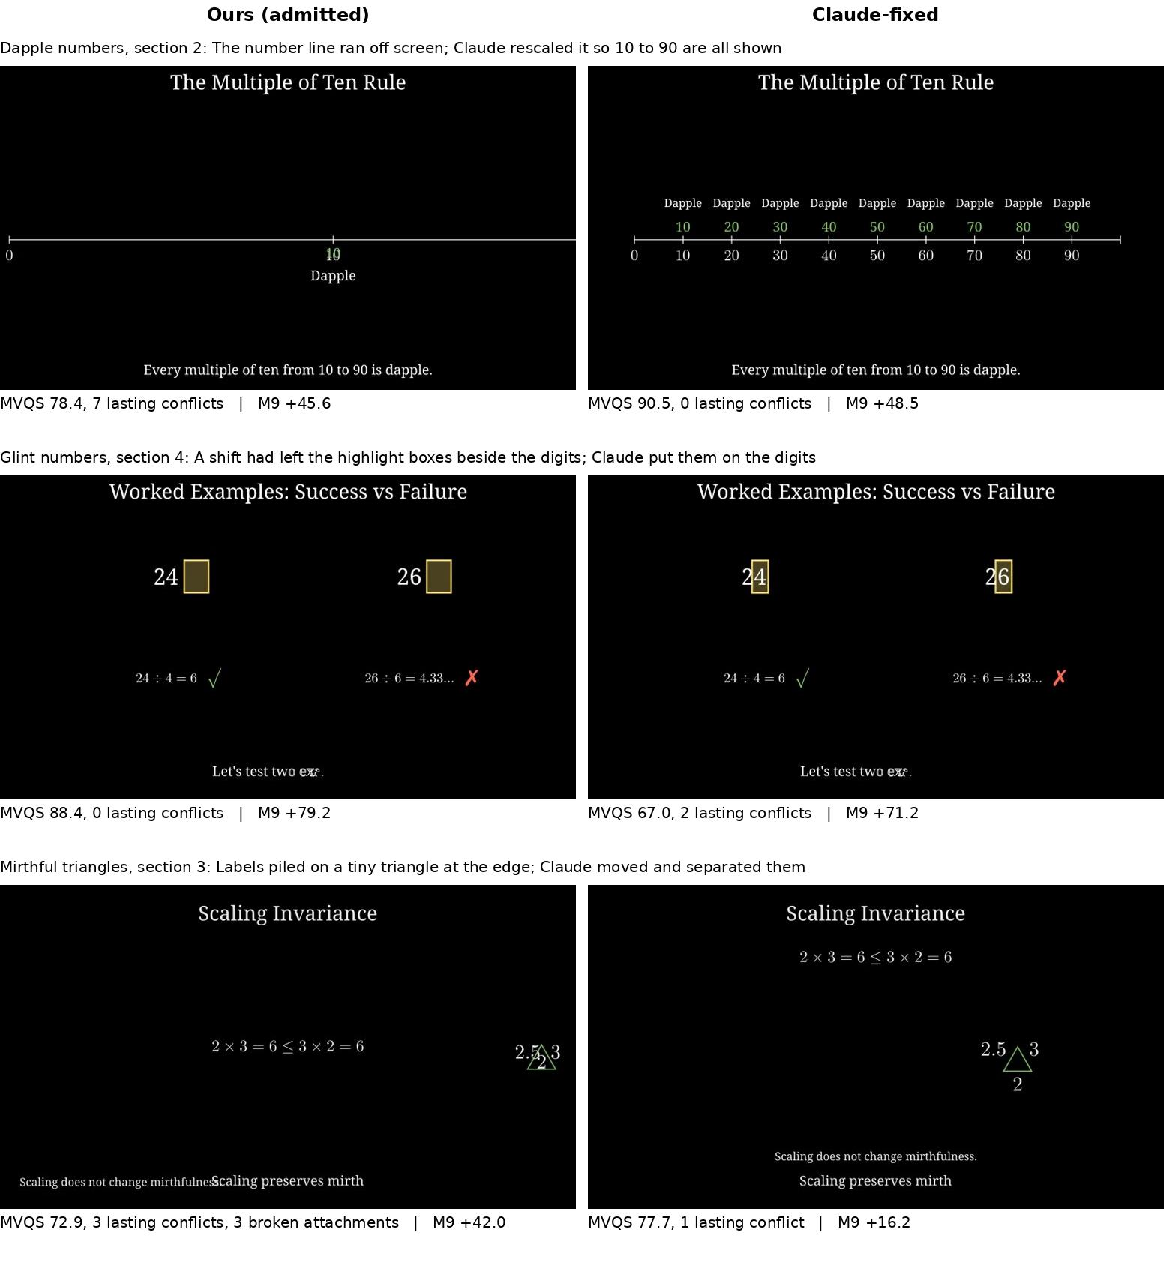
\includegraphics[width=\textwidth]{figures/layout_examples.pdf}
\caption{\textbf{The layout gets better; the score does not follow.} Three frames the student saw, from our admitted
video (left) and the Claude-fixed video (right). Under each frame: that section's layout score (MVQS), lasting
conflicts and broken attachments, then M9 for the whole concept (all four sections; \texttt{gemma4:26b}). Top: the
number line ran off screen and only 0 and 10 were visible. The fix shows 10 to 90, MVQS rises by 12 points, and M9
barely moves. Middle: a shift had left the highlight boxes over empty space beside the digits. The fix puts them on
the digits, which MVQS counts as two conflicts, so MVQS falls by 21 points although the frame is clearer. Bottom: labels
piled on a tiny triangle at the edge, and two captions collided. The fix separates them; MVQS rises a little, and M9
falls by 26 points. No single concept's change in M9 is beyond noise (Section~\ref{sec:results}).}
\label{fig:layout_examples}
\end{figure*}

\paragraph{Pipeline ablation} (Table~\ref{tab:stages}). All six stages (\S\ref{sec:ablation}) are scored on the
admitted NOVEL-12 concepts. The first stage, F0, is the pilot's loop. Its learner repair scores \NMRepair{} points of
M9 above the base video, ahead on \NMRepairPos{} of \NMRepairN{} concepts, and \NMRepairGeneric{} points above the
generic repair of the same size. Neither difference is beyond noise. Four insights follow from the later stages.
(i) \textbf{No feature makes the student's answers count.} By the rule fixed in advance, a feature helps if it
raises the learner repair's lead over the generic repair. From F1 to F5 that lead is \NMStageOneGeneric{},
\NMStageTwoGeneric{}, \NMStageThreeGeneric{}, \NMStageFourGeneric{} and \NMStageFiveGeneric{} points, against
\NMRepairGeneric{} at F0. Finding the weak section (F3) also does not beat rewriting every section beyond noise.
(ii) \textbf{The enforced gate keeps few revisions.} From F1 on, a revision that fails the gate is not used, and TEST
sees the base video instead. The gate kept the learner revision on only 1 to 5 of the 10 concepts per stage. So most
of each stage's learner videos are the base video.
(iii) \textbf{Kept revisions help on the 3 frames, not on the dense video.} The learner repair scores
\NMStageOne{}, \NMStageTwo{}, \NMStageThree{}, \NMStageFour{} and \NMStageFive{} points of M9 above the base video at
F1 to F5. Of the 17 revisions the gate kept, 16 raised M9. On the dense video (M7), the learner repair is at or below
the base video at every stage. Some gains rest on very little: on \emph{Tovan sums}, every kept revision fixes the same
single answer.
% Hand-counted from bench/results/noise-model/report.json (R1..R5, non-zero per-topic values: 17, of which 16 > 0);
% M7 learner - base and the edit sizes from bench/results/novel12-stages/report.md.
(iv) \textbf{None of these differences is beyond noise.} Four pass the question-swap test: F2, F3 and F5 against
the base video, and F5 against the generic repair. None holds across concepts, and none can: that test needs at least
six concepts to change in the same direction, and the gate let at most five change. Allowing for the ten stage
comparisons, none passes the question-swap test either. F3's difference comes from a single concept.
Two features do what they were built for. Checking the code before rendering (F2) raised the rewritten sections that
rendered from 25 to 28 of 32. Small edits (F5) change about 23\% of a section's lines, against about 70\% for the
rewrites of F2--F4. The edits did not keep the layout clean, though. The gate lets a revision lower the layout
score by up to 5 points and checks nothing else about the layout. In \RLWorse{} of the \RLRevisions{} revisions the F5 gate kept, the
edit added lasting conflicts or broken attachments. Over these \RLRevisions{}, lasting conflicts rose from
\RLConflictsBase{} to \RLConflictsLearner{} and broken attachments from \RLAttachBase{} to \RLAttachLearner{}
(\texttt{bench/repair\_layout.py}). So on NOVEL-12, with this student, the repair loop gives no gain
beyond noise at any stage. With ten concepts and most revisions refused, small benefits could not have been detected.

\begin{table*}[!tbp]\centering\small
\caption{Effect of each pipeline feature on NOVEL-12. Features are added one at a time; the base video is the same in every row. Gain: share of what the student did not know that it learned from 3 frames per section (version M9), in points. Learner $-$ generic: the learner repair against an equally large repair without the student's signal, scored on 3 frames (M9) and on the dense video (M7); small numbers: change against the row above. Layout: MVQS of the learner videos. Rewritten: sections rewritten and rendered. Used: topics whose final video is the revision.}\label{tab:stages}
\begin{tabular}{lrrrrrrrrr}\toprule & \multicolumn{4}{c}{Gain ($\uparrow$)} & \multicolumn{2}{c}{Learner $-$ generic ($\uparrow$)} & & & \\
\cmidrule(lr){2-5}\cmidrule(lr){6-7}
Stage & Base & Generic & Every section & Learner & 3 frames & Dense & Layout ($\uparrow$) & Rewritten & Used\\\midrule
F0: pilot loop & 42.4 & 42.4 & 38.9 & 48.5 & +6.1 & +3.4 & 81.3 & 25 & 10/10 \\
+ keep only revisions that pass the check & 42.4 & 44.5 & 45.2 & 50.2 & +5.6\worse{$-$0.5} & $-$3.7 & 84.5 & 25 & 5/10 \\
+ check the code before rendering & 42.4 & 51.2 & 42.2 & 54.6 & +3.4\worse{$-$2.2} & $-$5.4 & 84.2 & 28 & 4/10 \\
+ find the weak section like a debugger & 42.4 & 43.7 & 43.4 & 45.9 & +2.1\worse{$-$1.3} & $-$3.0 & 84.9 & 10 & 1/10 \\
+ block fixes that copy the practice quiz & 42.4 & 42.9 & 46.3 & 44.9 & +2.0\worse{$-$0.1} & $-$1.4 & 84.3 & 8 & 3/10 \\
+ small edits instead of rewrites & 42.4 & 42.2 & 42.8 & 48.5 & +6.3\better{+4.3} & $-$4.1 & 84.4 & 9 & 4/10 \\
\bottomrule\end{tabular}
\end{table*}

